\documentclass[12pt, a4paper]{article}
\usepackage[utf8]{inputenc}
\usepackage[IL2]{fontenc}
\usepackage[czech]{babel}
\usepackage{graphicx}

\begin{document}
\begin{figure}[h!]
\centering

\includegraphics[bb= 0 0 820 445 , width=75mm]{favlogo.jpg}
\end{figure}

\vspace{5cm}

{\centering
{\huge Architektura CRCE}\\[1em]
{\large KIV/SAR - semestrální práce}\\[7,5cm]
}

\begin{tabular}{l r}
student: & Radek VAIS, Zdeněk VALEŠ\\
mail: & vaisr@students.zcu.cz, valesz@students.zcu.cz\\
datum: & 1.1.2019\\
\end{tabular}

\thispagestyle{empty}
\newpage

%========================================
%========================================
%========================================
%========================================
%========================================
\section{Zadání} %=====================================================================================================

CRCE\footnote{Component Repository supporting Compatibility Evaluation} je komponentívé úložiště vyvíjené v rámci výzkumu na Katedře informatiky a výpočetní techniky na Západočeské univerzitě v Plzni. Jeho hlavní vlastností je podpora kontroly kompatibility verzí různých OSGi komponent nebo webových api.

\subsection{Motivace}

Vývoj projektu probíhá již několik let a vystřídalo se na něm mnoho vývojářů, což způsobilo zanesení větších či menších architektonických dluhů. Projekt již můžeme klasifikovat jako velký. Existuje potřeba, aby střídající se vývojáři (např. v rámci bakalářských prací) snadno a rychle zprovoznili základní instalaci a získali tak prostředí, pro rychlý vývoj nových částí. 

\subsection{Cíle projektu}

\begin{itemize}
	\item Unifikovat proces sestavení aplikace a spuštění.
	\item Zdokumentovat současnou architekturu aplikace.
	\item Analyzovat závislosti modulů v projektu a ověřit, zda některé moduly mají být součástí jádra.
	\item Připravit Docker image pro vývojáře.
\end{itemize}

\newpage
%========================================
%========================================
%========================================
%========================================
%========================================
\section{Analýza~architektury} %============================================================================================

Celý projekt je rozdělen do čtyř hlavních modulů: sdílené nastavení sestavení, jádro, moduly a knihovny třetích stran. Ne zcela jasné je začlenění modulů pro nasazení mezi moduly CRCE. závislostí modulů na jádře pozorujeme dva typy deklarování závislostí. Prvním způsobem je závislost na agregačním modulu jádra, druhým je jmenovitá závislost na komponentách jádra. Tyto skutečnosti jsou patrné na celkovém diagramu na Obrázku \ref{fig:wholeCRCE}.

\begin{figure}[h!]
\centering
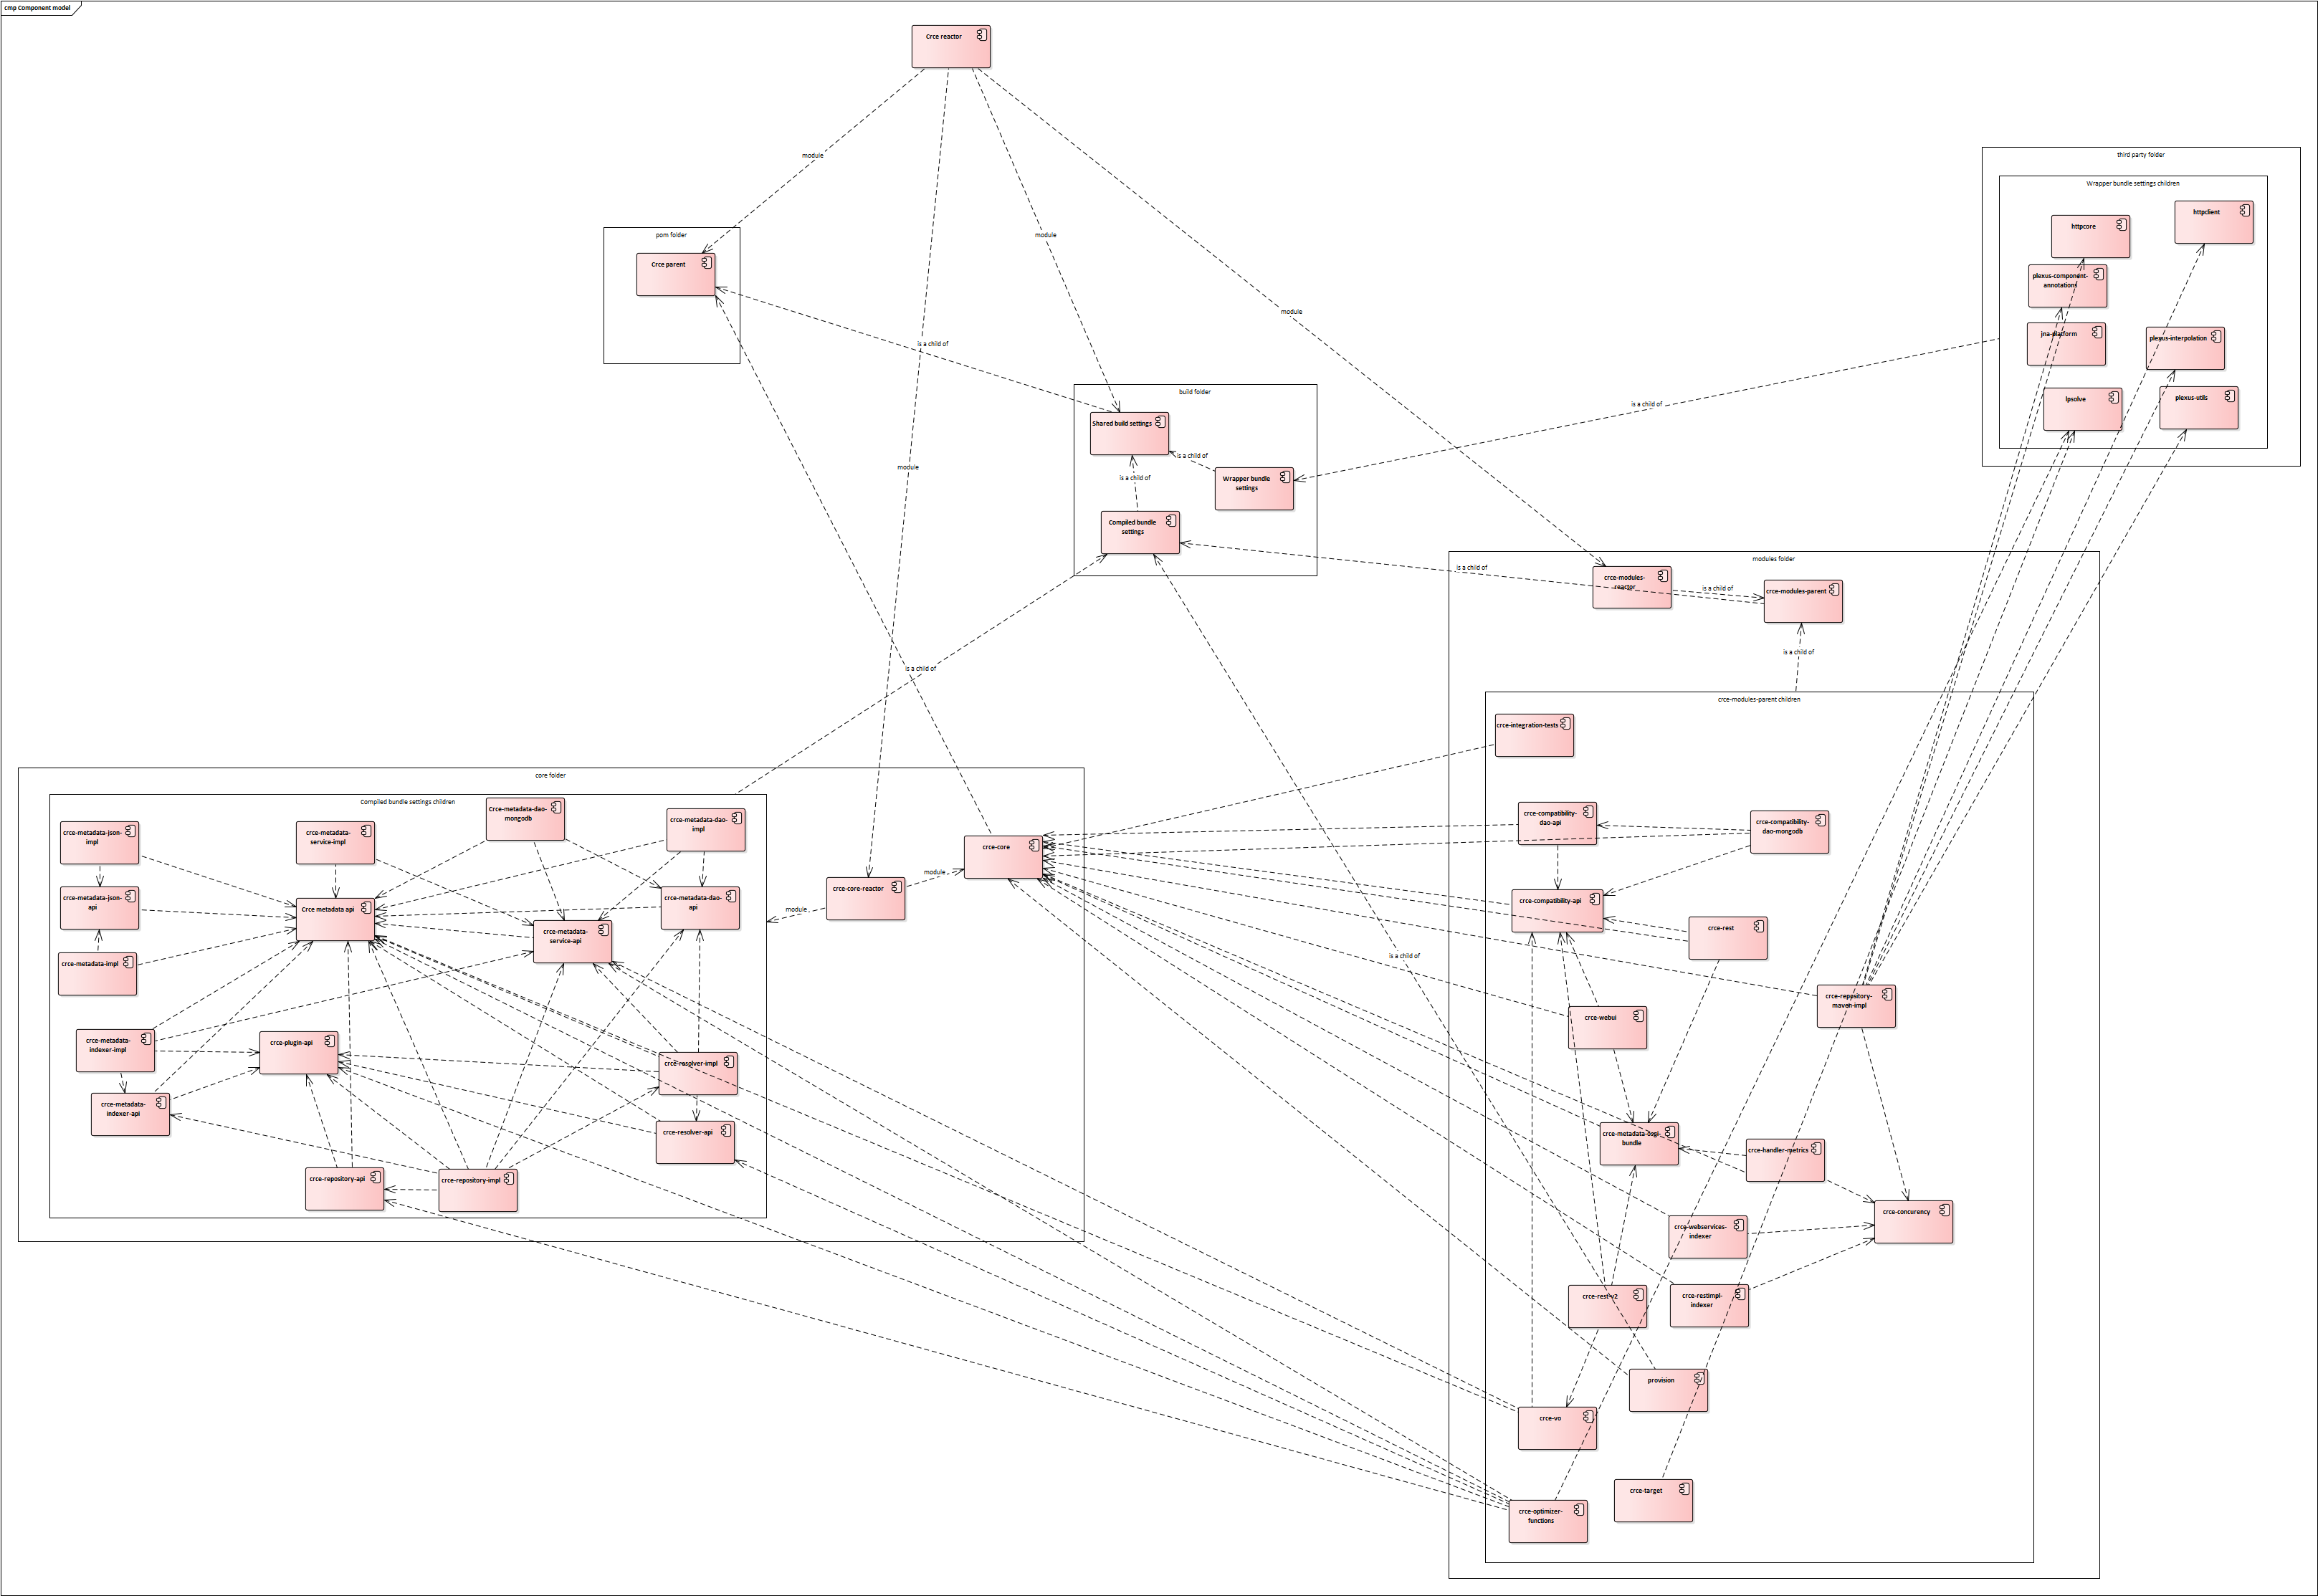
\includegraphics[width=135mm]{wholeCRCE.png}
\label{fig:wholeCRCE}
\caption{Diagram závislostí všech maven komponent projektu CRCE před provedenými úpravami.}
\end{figure}

Během analýzy modulu pro moduly CRCE jsme identifikovali několik kandidátů na přesun do jádra. Za kandidáty jsme volili takové komponenty, které využívá velká část ostatních modulů a zároveň tyto moduly mají závislosti do jádra. Tomuto pravidlu odporuje komponenta webového rozhraní, bez kterého úložiště nelze použít. Přesouvané komponenty jsou: crce-compatibility-api, crce-webui, crce-concurency (graficky znározněno na Obrázku \ref{fig:modulesCRCE}. 

Po identifikace kandidátů jsme z přesunu vyřadili komponentu metadata-osgi-bundle, protože není dostatečně obecná. Komponenta indexuje pouze OSGi komponenty. Bohužel přesouvaná komponenta webui obsahuje nevhodnou závislost na této komponentě. Tato závislost jde proti snadné záměně komponenty pro indexaci vstupů úložiště. Navrhli jsme tedy přidání metody do rozhraní indexeru pro zjištění jaké elementy indexer zpracovává.

\begin{figure}[h!]
\centering
\includegraphics[width=135mm]{modules.png}
\label{fig:modulesCRCE}
\caption{Diagram původních závislostí uvnitř mudulu moduly CRCE. Zeleně jsou označeny přesouvané komponenty. Červeně je označena nevhodná závilsost.}
\end{figure}

%========================================
%========================================
%========================================
%========================================
%========================================
\section{Provedené~změny} %=======================================================================================

\begin{itemize}
	\item Oddělení modulů pro spuštění CRCE do nového modulu deploy.
		\subitem Vytvoření komponenty default-modules, která zachycuje verze spouštěných modulů.
	\item Přesun komponent crce-compatibility-api, crce-webui, crce-concurency do jádra CRCE.
		\subitem Vytvoření testů vlastností a defaultních rozhraní.
		\subitem Rozšíření rozhraní indexerů.
	\item Dokerizace základní instance CRCE.
		\subitem Konfigurace DB connection pomocí proměnných prostředí (oddělení DB).
		
\end{itemize}

%========================================
%========================================
%========================================
%========================================
%========================================
\section{Uživatelská~příručka} %======================================================================================

Provedené změny ovlivnily základní používání projektu při vývoji. 

Pro sestavení na platformě Linux lze použít bash script build.bash, který automaticky spustí jednotlivé kroky sestavení pomocí programu Maven.

Nastavení connection stringu je možné pomocí proměnné prostředí \texttt{mongo\_connection}. Příkladem takového parametru je: \emph{mongodb://localhost:27017}.


%========================================
%========================================
%========================================
%========================================
%========================================
\newpage
\section{Závěr}  %======================================================================================================

V rámci projektu jsme naplnili cíl usnadnit novým vývojářům spuštění výchozí aplikace, především přípravou docker image. Nepodařilo se nám zjednodušit proces sestavení celé aplikace na jeden Maven příkaz nicméně pro prostředí Linux jsme vytvořili script, který úkony nutné pro sestavení provede automaticky.
Dále jsme přesunuli několik modulů do jádra CRCE z důvodu jejich provázanosti s ostatními nebo nutnosti pro používání. 


\end{document}